\documentclass[12pt,a4paper]{article}
\usepackage{tikz}
\usepackage{pgfplots}
\pgfplotsset{compat=1.18}
\usetikzlibrary{arrows.meta, positioning, shapes.geometric}
\usepackage{geometry}
\usepackage[T1]{fontenc}
\usepackage{titlesec}
\usepackage{tabto}
\usepackage[most]{tcolorbox}
\usepackage{xcolor}
\usepackage{lscape}
\usepackage{amsmath,amssymb}
\usepackage[colorlinks=true,linkcolor=blue]{hyperref}
\geometry{margin=2.0cm}

\definecolor{highcolor}{RGB}{45,152,222}
\newcommand{\highlight}[1]{{\color{highcolor}{\textbf{#1}}}}
\newcommand{\sansbold}{\usefont{T1}{lmss}{b}{n}\selectfont}
\tcbset{
  notebox/.style={
    colback=highcolor!8, 
    colframe=highcolor!45,
    coltitle=blue!70!black, % dark blue title
    arc=4pt, 
    boxrule=0.6pt,
    left=6pt, right=6pt, top=5pt, bottom=5pt,
    toptitle=4pt, bottomtitle=4pt,
    fonttitle=\sansbold,
  }
}

% make highlight with paragraph and noindent
\newcommand{\highlightnew}[1]{\vspace{0.3cm}\par\noindent\highlight{#1}}

\newcommand\skipsectionnumber{\tabto{0.5cm}}
\newcommand\skipsubsectionnumber{\tabto{1cm}}

\titleformat{\section}[hang]
  {\usefont{T1}{lmss}{b}{n}\selectfont\large}
  {\thesection.}
  {.5em}
  {\skipsectionnumber}

\titleformat{\subsection}[hang]
  {\usefont{T1}{lmss}{b}{n}\selectfont\normalsize}
  {\thesubsection}
  {.5em}
  {\skipsubsectionnumber}


\newcommand{\params}{Y}
\newcommand{\paramsi}{\params_i}
\newcommand{\datanoisy}{Z}
\newcommand{\datanoisyi}{\datanoisy_i}
\newcommand{\hyperparams}{X}
\newcommand{\hiddenparams}{Y}
\newcommand{\hiddenparam}[1]{Y_{#1}}         % single hidden param
\newcommand{\Lik}{\mathcal{L}}
\newcommand{\prior}{p}
\newcommand{\dd}{\mathrm{d}}
\newcommand{\erf}{\text{erf}}
\usetikzlibrary{
  positioning, arrows.meta, fit,
  decorations.pathreplacing, backgrounds, calc
}


% ── colour palette ────────────────────────────────────────────────────────────
\definecolor{popclr}   {HTML}{6A4C93}
\definecolor{hidclr}   {HTML}{2A9D8F}
\definecolor{dataclr}  {HTML}{E76F51}
\definecolor{ppclr}    {HTML}{F4A261}
\definecolor{boxbg}    {HTML}{F8F9FA}
\definecolor{arrowclr} {HTML}{444444}

% ── helper styles ─────────────────────────────────────────────────────────────
\tikzset{
  mybox/.style={
    draw=#1, fill=boxbg, rounded corners=4pt,
    inner sep=6pt, line width=0.8pt
  },
  colhead/.style={font=\bfseries\small, text=#1},
  arr/.style={-Stealth, thick, color=arrowclr,
              shorten >=4pt, shorten <=4pt},
  plotbox/.style={mybox=#1, minimum width=3.2cm, minimum height=2.6cm},
  sublabel/.style={font=\footnotesize, text=#1},
}



% ── column x-positions ───────────────────────────────────────────────────────
\newcommand{\colA}{0cm}
\newcommand{\colB}{5.6cm}
\newcommand{\colC}{11.2cm}

% ── row y-positions (headers at 0, plots below, inference further below) ─────
\newcommand{\rowHead}{0cm}
\newcommand{\rowOne}{-1.4cm}
\newcommand{\rowTwo}{-6.8cm}

\title{{\usefont{T1}{lmss}{b}{n}\selectfont\LARGE Introduction to Hierarchical Bayesian Analysis}}
\author{}
\date{}

\begin{document}
\maketitle

\section{Motivation}

Make general statements about a population of objects, given a limited set of observed data points.



\subsection{Reminder}


The posterior is given by
\[
  p(\hyperparams\mid\datanoisy)\;\propto\;
  \underbrace{p(\datanoisy\mid\hyperparams)}_{\text{Likelihood}}\;
  \underbrace{p(\hyperparams)}_{\text{Prior}}
  \,,
\]
where $\hyperparams$ are the population-level parameters of interest and $\datanoisy$ is the data. 
In hierarchical Bayesian inference, the data is structured, i.e.
\[
  \datanoisy \;\longrightarrow\; \{\datanoisy\} = \{\datanoisy_1,\, \datanoisy_2,\, \ldots,\, \datanoisy_N\}
\]
with repeated measurements (not necessarily of the same quantity). 
%
So that the relevant posterior becomes
\[
  p(\hyperparams\mid\{\datanoisy\}) \propto p(\{\datanoisy\}\mid\hyperparams) p(\hyperparams)
\]


\subsection{Naming convention}

I will call the population-level parameters $X$, the hidden parameters $Y$, and the data $Z$.
Examples for population-level parameters are the maximum of a distribution, or the slope of a line. 
Examples for hidden parameters are the true value of a measurement, say the mass of a star (so not directly observed). 
Examples for data a time series, a spectrum, an image, etc. 








\subsection{Estimating the maximum of a uniform distribution}

We are given $N$ data points $\paramsi$ drawn from a uniform distribution $\mathcal{U}(0, M)$, where $M$ is an unknown parameter we want to estimate.
For the three independent draws $4.24, 0.95, 6.68$, what is the best estimate for $M$?

\highlightnew{Intuition.}
The maximum of the distribution must be at least as large as the largest observed data point, so the posterior of $M$ must be zero for $M < 10.2$.
The maximum cannot be too large either, otherwise the observed data points would be very unlikely (to be so small). 
Somewhat, the posterior support close to $M$ is determined by how data points one has observed.

\highlightnew{Computation. }
For one draw, we have $p(\paramsi \mid M) = \frac{1}{M}\Theta_{[0,M]}(\paramsi)$, where $\Theta$ is the Heaviside step function.
For $N$ independent draws, we have
\[
    p(\{\params\} \mid M) = \prod_{i=1}^{N} p(\paramsi \mid M) = \frac{1}{M^N}\prod_{i=1}^{N} \Theta_{[0,M]}(\paramsi)
    \,.
\]
Exploiting that the product of Heaviside functions is zero if $M$ is smaller than the largest data point, and one otherwise, we have
\[
    p(\{\params\} \mid M) = \frac{1}{M^N}\Theta_{[\max_i \paramsi,\infty)}(M)
    \,.
\]
Assuming a uniform prior $p(M) \propto 1$, the posterior is 
\[
    p(M \mid \{\params\}) \propto p(\{\params\} \mid M) p(M) = \frac{1}{M^N}\Theta_{[\max_i \paramsi,\infty)}(M)
    \,.
\]
The posterior is a power law with support only for $M$ larger than the largest data point, and the maximum a posteriori (MAP) estimate is $\hat{M} = \max_i \paramsi$.
See Fig.~\ref{fig: example uniform distribution} for an example with the three data points (\textit{left}) and varying number of data points (\textit{right}).

\begin{figure}[ht]
    \centering
    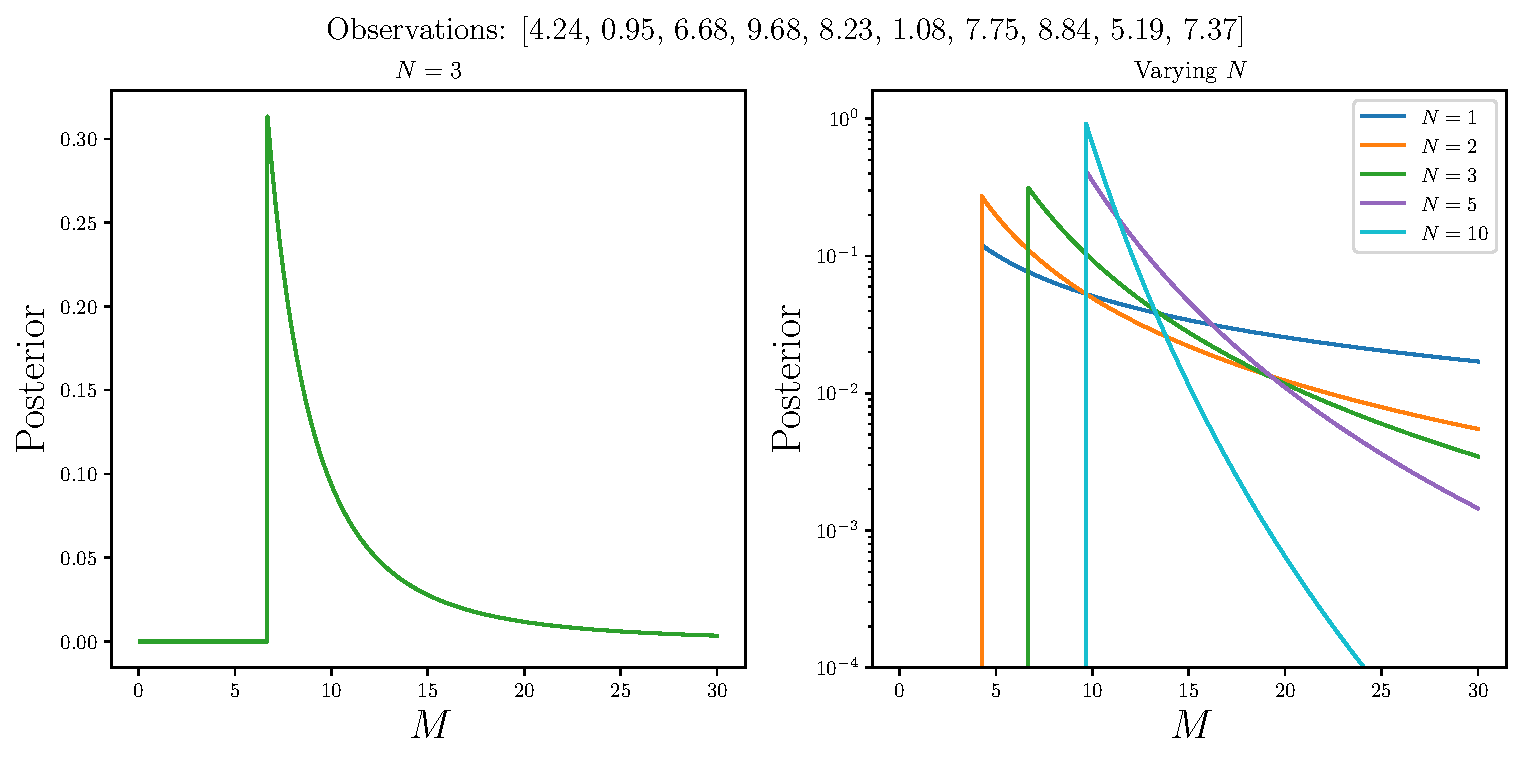
\includegraphics[width=\textwidth]{notebooks/plots/example_uniform_distribution_varying_N.pdf}
    \caption{Posterior distribution of $M$ given three data points drawn from $\mathcal{U}(0,M)$ (\textit{left}) and varying number of data points (\textit{right}). }
    \label{fig: example uniform distribution}
\end{figure}


\begin{tcolorbox}[notebox, title={Summary}]
\begin{itemize}
    \item Easy since the one-dimensional likelihood depends only on the maximum of the data. 
    \item The uncertainties shrink with more data points. 
    \item As in almost all Bayesian inference, the posterior has different structure that the likelihood. 
    \item This is ``as good as it gets'', for independent draws from a uniform distribution, this is the PDF over the maximum of that distribution. 
    \item Example for a posterior that never approaches a Gaussian, even for the number of data points going to infinity.
    \item The estimated maximum is uncertain because there are two types on ``noise'', here this is Poisson noise! (We will get to noise on the parameters in the next example).
\end{itemize}
\end{tcolorbox}

\begin{tcolorbox}[notebox, title={Question}]
\begin{itemize}
    \item How would the power-law exponent change for correlated data points?
\end{itemize}
\end{tcolorbox}

\subsection{Estimating the maximum of a uniform distribution, with noise}

\highlightnew{How will uncertain observations change the posterior?}
Say, we have no direct access to $\params$, but only to a noisy version $\datanoisy = \params + \varepsilon$, where $\varepsilon$ is a zero-mean Gaussian noise with known standard deviation $\sigma$.
The single likelihood of observation is 
\begin{align}
    p(\datanoisyi \mid M)
    &= \int p(\datanoisyi, \paramsi \mid M) \, \dd \paramsi \nonumber \\ 
    &= \int p(\datanoisyi \mid \paramsi) p(\paramsi \mid M) \, \dd \paramsi \nonumber \\ 
    &= \int \frac{1}{\sqrt{2\pi}\sigma} e^{-\frac{1}{2\sigma ^ 2}(\datanoisyi - \paramsi)^2} \frac{1}{M}\Theta_{[0,M]}(\paramsi) \, \dd \paramsi \nonumber \\
    &= \frac{1}{M \, \sqrt{2\pi}\sigma} \int \Theta_{[0,M]}(\paramsi) e^{-\frac{1}{2\sigma ^ 2}(\datanoisyi - \paramsi)^2} \, \dd \paramsi \nonumber \\
    &= \frac{1}{2M} \left[
        \text{erf}\left(\frac{M - \datanoisyi}{\sqrt{2}\sigma}\right) - \text{erf}\left(\frac{-\datanoisyi}{\sqrt{2}\sigma}\right)
    \right] \nonumber \\
    &= \frac{1}{2M} \left[
        \text{erf}\left(\frac{M - \datanoisyi}{\sqrt{2}\sigma}\right) + \text{erf}\left(\frac{\datanoisyi}{\sqrt{2}\sigma}\right)
    \right]
    \,.
\end{align}
%
Under the independence assumption of noise realization and parameters $\params$, the likelihood of $N$ independent observations is again just the product of the single likelihoods. 
Fig.~\ref{fig: example uniform distribution noisy} shows the posterior of $M$ given the same three data points as before, but now assuming these data points include noise.

\begin{figure}[ht]
    \centering
    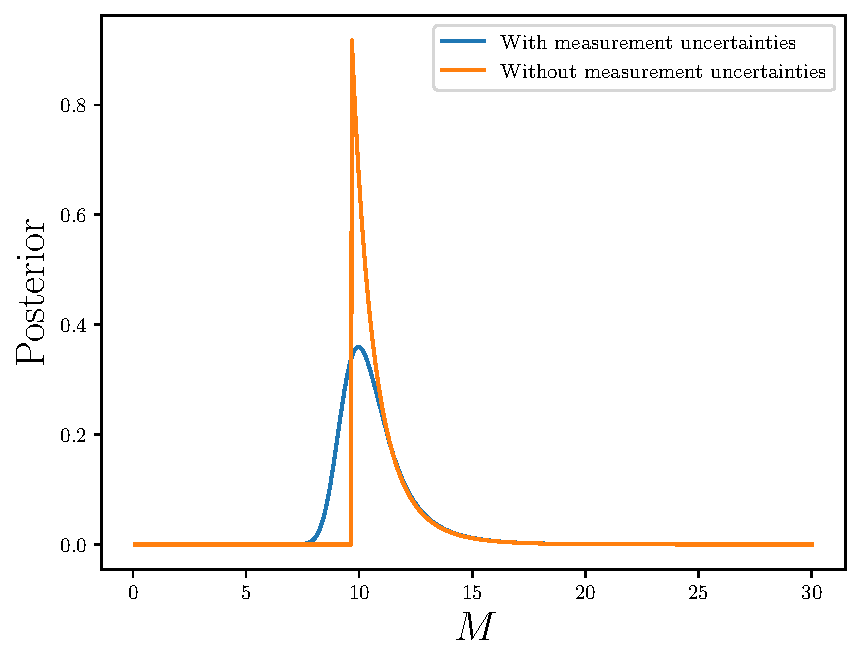
\includegraphics[width=0.7\textwidth]{notebooks/plots/example_uniform_distribution_noisy.pdf}
    \caption{Posterior distribution of $M$ given three noisy data points, with $\sigma = 1$. }
    \label{fig: example uniform distribution noisy}
\end{figure}


\begin{tcolorbox}[notebox, title={Summary}]
    \begin{itemize}
        \item Measurement uncertainties significantly smooth out the posterior (proportional to $\sigma$). 
        \item Compared to previously posterior depends on explicit value of \textit{all} points. The above case was a special case!
        \item For large $M$ (compared to the data points), behavior of $M ^ {- N}$ remains the same.
        \item For $\sigma \rightarrow 0$, the posterior approaches the case without noise (as expected).
        \item Example for overestimating the noise will bias the posterior towards smaller values of $M$. Overestimation of noise is thus not always conservative! 
        \item Special case: we could analytically marginalize over the hidden parameters $\params$ to obtain the likelihood of the data given $M$. For more realistic problems, this is not possible, and one has to approximate these integrals. 
    \end{itemize}
\end{tcolorbox}


\begin{tcolorbox}[notebox, title={Connection to astrophysics}]
In the above examples, the single-observation data was always only one number (or can be characterized by a small set of parameters such as the mean and standard deviation of a Gaussian), which makes the likelihood easy to compute.
In astrophysics, the data is high-dimensional, i.e.\ a spectrum, an image, a time series, etc. We will come back to this point later!
\end{tcolorbox}

\begin{tcolorbox}[notebox, title={Uncertainties}]
    In the above examples, the uncertainty on the single-observation level was (i) independent of the single-observation parameters and (ii) any other parameters (such as time of observation). 
    This made the population-level likelihood easy to compute, because one could ``forward-model'' the likelihood of the data directly. For real observations this is often not the case -- we will come back to the use of posterior samples later. 

    \vspace{0.2cm}
    In principle, if the noise if not known a priori, one could also infer the noise parameters (e.g. $\sigma$), making it part of the population-level parameters $\hyperparams$.
    However, often the noise is often characterized by previous experiments, and the uncertainties on the noise parameters are small compared to the uncertainties on the population-level parameters, so the uncertainty of the noise parameters is neglected. 
\end{tcolorbox}




\subsection{Estimating the maximum of a power-law distribution, no noise}

\highlightnew{Adding more parameters.}
Now there are two parameters to estimate: the maximum $M$ and the power-law exponent $\alpha$.
The likelihood becomes
\[
    p(\paramsi \mid M, \alpha) = \frac{(\alpha + 1)}{M^{\alpha + 1}}\Theta_{[0,M]}(\paramsi)\,\paramsi ^ {\alpha}
    \,.
\]
Again the likelihood of $N$ independent draws is just the product of the single likelihoods, and the posterior is given by the product of the likelihood and a prior.
We can simplify
\[
    p(\{\params\} \mid M, \alpha) = \prod_{i=1}^N p(\paramsi \mid M, \alpha) = \frac{(\alpha + 1)^N}{M^{N(\alpha + 1)}}\Theta_{[\max_i\paramsi, \infty]}(M)\,\prod_{i=1}^N \paramsi ^ {\alpha}
    \,.
\]
%
Fig.~\ref{fig: example power law distribution} shows the posterior of $M$ and $\alpha$ given varying number of data points drawn from a power-law distribution, with the true parameters indicated as a blue cross.

\begin{figure}
    \centering
    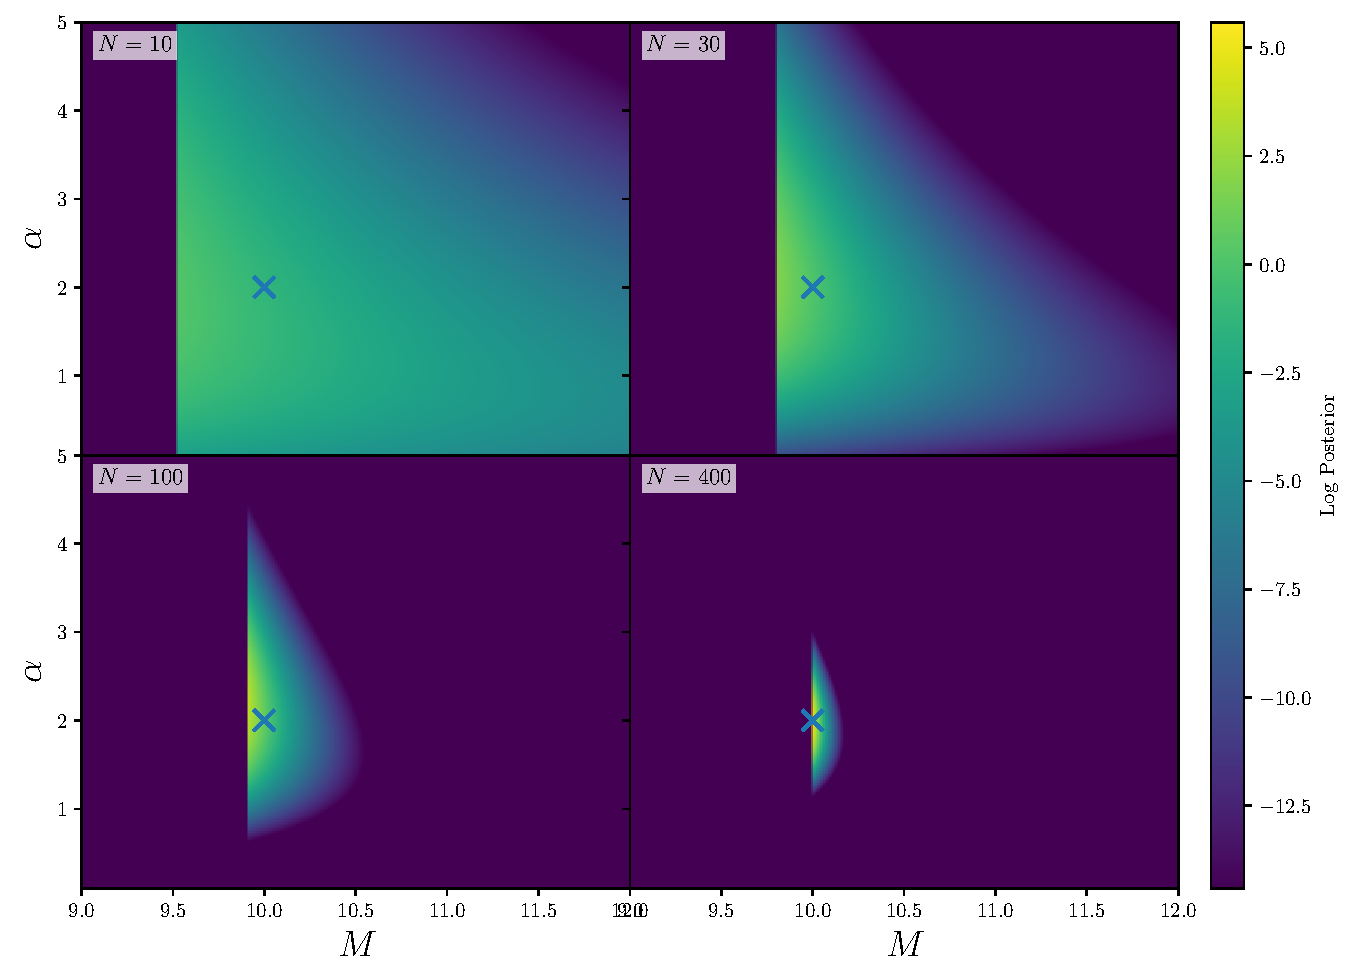
\includegraphics[width=\textwidth]{notebooks/plots/example_power_law_distribution_varying_N.pdf}
    \caption{Posterior distribution of $M$ and $\alpha$ given varying number of data points drawn from a power-law distribution, with the true parameters indicated as a blue cross. }
    \label{fig: example power law distribution}
\end{figure}

\begin{tcolorbox}[notebox, title={Summary}]
    \begin{itemize}
        \item Best-case scenario: see figure for best possible constraint given some observations (noise will only weaken constraints).
        \item Depending on $\alpha$, the decay of $M$ can be much faster than the uniform case (because large $\alpha$ means more data points close to the maximum. 
        The opposite is also true, for negative $\alpha$ the uncertainty decrease with the number of data points is slow\footnote{Note that in the case of $\alpha+1>0$, one has to introduce a minimum different from zero. }).
    \end{itemize}
\end{tcolorbox}


\subsection{Example: fitting a line}

Say for fixed and known $x_i$, we have noisy observations $\datanoisyi = \hiddenparam{i} + \varepsilon_i$, where $\varepsilon_i$ is a zero-mean Gaussian noise with known standard deviation $\sigma$, for simplicity independent of the observation.
We want to fit a linear function through the origin, so the ``distribution'' of $\hiddenparam{i}$ given the population-level parameter $\hyperparams$ is simple
\[
    p(\hiddenparam{i} \mid \hyperparams) = \delta(\hiddenparam{i} - \hyperparams \cdot x_i)
    \,.
\]
So this is a new conceptual step, where the distribution now depends on some known variable $x_i$ (before the maximum was independent of the observation, but you could easily imagine that the maximum also dependent on the number of data points, for example).

The likelihood of the data given the hidden parameters is
\[
    p(\datanoisyi \mid \hiddenparam{i}) = \frac{1}{\sqrt{2\pi}\sigma} e^{-\frac{1}{2}\left(\frac{\datanoisyi - \hiddenparam{i}}{\sigma}\right)^2}   
    \,.
\]
So one can actually analytically marginalize over the hidden parameters $\hiddenparam{i}$ to obtain the likelihood of the data given the population-level parameter $\hyperparams$
\begin{align}
    p(\datanoisyi \mid \hyperparams) &=
    \int p(\datanoisyi , \hiddenparam{i} \mid \hyperparams) \, \dd \hiddenparam{i} \nonumber \\
    &= \int p(\datanoisyi \mid \hiddenparam{i}) \; p(\hiddenparam{i} \mid \hyperparams) \, \dd \hiddenparam{i} \nonumber \\
    &= \int \frac{1}{\sqrt{2\pi}\sigma} e^{-\frac{1}{2}\left(\frac{\datanoisyi - \hiddenparam{i}}{\sigma}\right)^2} \delta(\hiddenparam{i} - \hyperparams \cdot x_i) \, \dd \hiddenparam{i} \nonumber \\
    &= \frac{1}{\sqrt{2\pi}\sigma} e^{-\frac{1}{2}\left(\frac{\datanoisyi - \hyperparams \cdot x_i}{\sigma}\right)^2} \nonumber \\
    &= \frac{1}{\sqrt{2\pi}\sigma} e^{-\frac{x_i^2}{2\sigma^2 }\left(X - \frac{\datanoisyi}{x_i}\right)^2}
     \,.
\end{align}
So for known $\sigma$, the likelihood of the data given the population-level parameter $\hyperparams$ is just a Gaussian likelihood, with mean and standard deviation given by
\[
    \mu_i = \frac{\datanoisyi}{x_i} \quad\text{and}\quad \sigma_i = \frac{\sigma}{x_i}
    \,.
\]
This is exactly what one naively expects: the mean is centered around the slope of the single point, and the uncertainty is larger for smaller $x_i$.
For a set of independent observations, the likelihood always remains Gaussian, with the maximum likelihood estimate of $\hyperparams$ given by the weighted means of the single-point estimates $\datanoisyi / x_i$.



\begin{center}
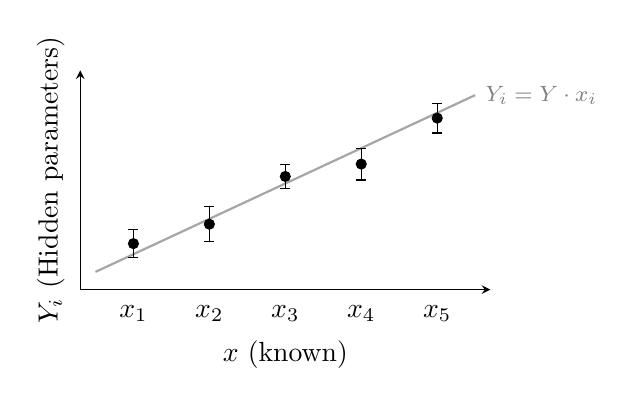
\begin{tikzpicture}
\begin{axis}[
  width=0.56\linewidth, height=0.36\linewidth,
  xlabel={$x$ (known)}, ylabel={$\hiddenparam{i}$ (Hidden parameters)},
  axis lines=left, tick style={draw=none},
  xtick={1,2,3,4,5},
  xticklabels={$x_1$,$x_2$,$x_3$,$x_4$,$x_5$},
  ytick=\empty,
  xmin=0.3, xmax=5.7, ymin=0, ymax=6.2,
  clip=false,
]
  % True linear relation
  \addplot[gray!70, thick, domain=0.5:5.5, samples=2] {x}
    node[right, font=\footnotesize, gray] {$\hiddenparam{i}=\params\cdot x_i$};

  % Noisy observations with error bars on Y
  \addplot[
    only marks, mark=*, mark size=1.8pt,
    error bars/.cd, y dir=both, y explicit,
  ] coordinates {
    (1, 1.3)  +- (0, 0.40)
    (2, 1.85) +- (0, 0.50)
    (3, 3.2)  +- (0, 0.35)
    (4, 3.55) +- (0, 0.45)
    (5, 4.85) +- (0, 0.42)
  };

%   \node[anchor=west, font=\footnotesize] at (axis cs:3, 3.2)
    % {\;$Y_i = \hiddenparam{i} + \varepsilon_i$};
\end{axis}
\end{tikzpicture}
\end{center}

\begin{tcolorbox}[notebox, title={Comment}, title filled=false, colframe=highcolor!45]
    In almost all cases, when fitting a line one does not compute $p(\datanoisyi \mid \hyperparams)$, solves first for the single-point estimates for $\hiddenparam{i}$, and then uses these estimates to compute the likelihood of the data given the population-level parameters $\hyperparams$.
\end{tcolorbox}



\begin{tcolorbox}[notebox, title={Product of population-level posterior from one observation}, title filled=false, colframe=highcolor!45]
In a significant portion of hierarchical Bayesian inference, the population-level posterior is just the product of the single-observation posteriors (and assumptions of independence of data and hidden parameters).
%  i.e.~there is not more information in the population-level posterior than in the set of 
Often, it is enough to understand the population-level posterior for a single observation to understand the population-level posterior given a set of observations.
\end{tcolorbox}


\subsection{Selection effects - no noise}
Selection effects are ubiquitous in science, and reflect the fact that the distribution of observed data points is not the same as the distribution of all data points. 
Examples are (i) bright stars are over-represented in a survey since they can be detected to larger distances, (ii) planets with short orbital periods are over-represented in transit surveys since they transit more often and the light curve is more affected in amplitude, (iii) waiting until one sees a five-sigma outlier before writing a paper, etc. 

For simplicity we consider again the uniform example, where the true distribution of parameters is uniform, i.e.~$p(\params\mid M) = \frac{1}{M}\Theta_{[0,M]}(\params)$, but we only observe data points that are larger than some threshold $C$.
For a single observation, one can thus consider that we draw from the uniform distribution until $\params > C$.
The likelihood of the data given $M$ is then
\[
    p(\paramsi \mid M, \params > C) = \frac{1}{M - C}\Theta_{[C,M]}(\paramsi)
     \,.
\]
Of course, this is just the same if we had considered the data being conditioned on being larger than $C$ from the beginning, i.e.~$p(\params\mid M, \params > C) = \frac{1}{M - C}\Theta_{[C,M]}(\params)$.
So with a on-off selection function, the likelihood is the same as above in the uniform case, but with with a minimum of $C$ (instead of zero).
Rewriting the above likelihood gives
\[
    p(\paramsi \mid M, \params > C) = \frac{1}{M - C}\Theta_{[\paramsi, \infty]}(M)
    % \quad \quad \text{for } M > C 
    \,.
\]
So this time the tail behavior is $(M - C) ^ {- N}$ for $N$ the number of observations (but of course this is the same as before, since $C = 0$ in the previous example).


\subsection{Selection effects - noise}

Say now we have noisy parameters, that again are related to the hidden parameters as $\datanoisy = \params + \varepsilon$, where $\varepsilon$ is a zero-mean Gaussian noise with known standard deviation $\sigma$.
Furthermore, we only include data points that are larger than some threshold $C$, so $\datanoisy > C$.

The likelihood of the data given $M$ is then
\begin{align}
    p(\datanoisyi \mid M, \datanoisy > C)
    &= \int p(\datanoisyi, \paramsi \mid M, \datanoisy > C) \, \dd \paramsi \nonumber \\ 
    &= \int p(\datanoisyi \mid \paramsi, \datanoisy > C)\, p(\paramsi \mid M)\, \dd \paramsi \nonumber \\ 
    &= \int 
    \frac{
      \frac{1}{\sqrt{2\pi}\sigma}
      \exp\!\left[-\frac{1}{2\sigma ^ 2}(\datanoisyi - \paramsi)^2\right]
    }{
      P(\datanoisy > C \mid \paramsi)
    }\;
    \frac{1}{M}\Theta_{[0,M]}(\paramsi)\, \dd \paramsi
    \nonumber \\
    &=
    \int 
    \frac{
      \frac{1}{\sqrt{2\pi}\sigma}
      \exp\!\left[-\frac{1}{2\sigma ^ 2}(\datanoisyi - \paramsi)^2\right]
    }{
        \frac{1}{2}\left[
            1 + \text{erf}\!\left(\frac{\paramsi - C}{\sqrt{2}\sigma}\right)
        \right]
    }\;
    \frac{1}{M}\Theta_{[0,M]}(\paramsi)\, \dd \paramsi
\end{align}
There is no analytical solution to this integral, so one has to compute it numerically.
For an example see Fig.~\ref{fig: example uniform distribution noisy selection}.

\begin{figure}
    \centering
    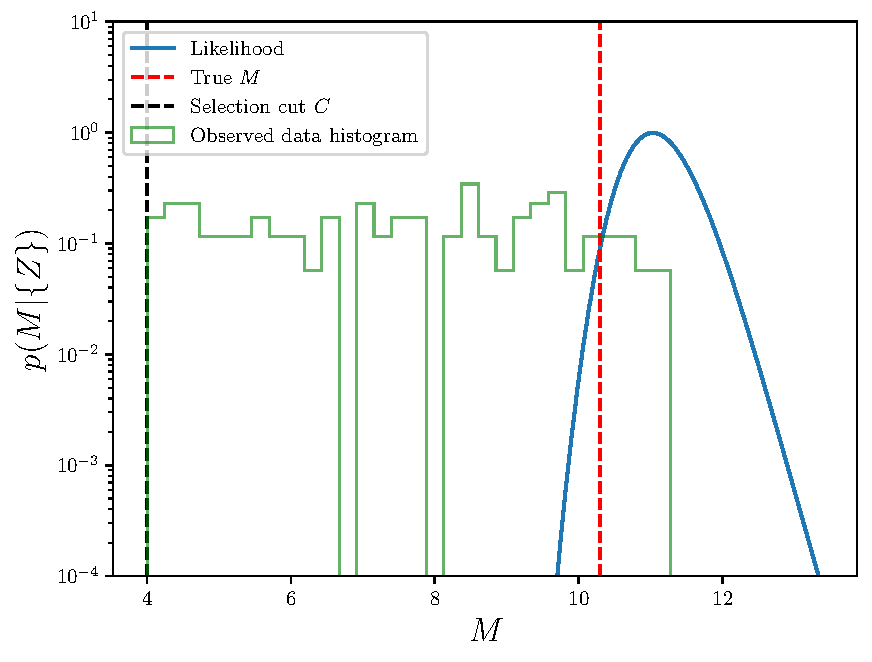
\includegraphics[width=0.7\textwidth]{notebooks/plots/selection_effect_with_noise_likelihood.pdf}
    \caption{Posterior distribution of $M$ given the selection-biased observations, with $\sigma = 1$ and a selection threshold of $C = 4$. }
    \label{fig: example uniform distribution noisy selection}
\end{figure}




\section{Problem formulation}


%──────── 2. Structured Data ─────────────────────────────────────────────────
\subsection{Structured Data --- Equal Footing}

\[
  \datanoisy \;\longrightarrow\; \{\datanoisy\} = \{\datanoisy_1,\, \datanoisy_2,\, \ldots,\, \datanoisy_N\}
\]
With repeated measurements (not necessarily of the same quantity). 
%
So that the relevant posterior becomes
\[
  p(\hyperparams\mid\{\datanoisy\}) \propto p(\{\datanoisy\}\mid\hyperparams) p(\hyperparams)
\]
Assume each data point $\datanoisyi$ is determined by a set of parameters we do not have direct access to. 
We will call these \emph{hidden parameters} $\hiddenparam{i}$.
The likelihood then becomes
\[
    p(\{\datanoisy\}\mid\hyperparams) \rightarrow p(\{\datanoisy\}, \{\hiddenparams\}\mid\hyperparams)
    \,,
\]
a very high-dimensional problem.
Note that a priori we need both the global parameters $\hyperparams$ and the hidden parameters $\hiddenparams$ to determine the likelihood of the data.
However, if one choses the hidden variables that describe the data without reference to the global parameters, then the likelihood can be factorised into a local and a global part. 
So, 
\[
    p(\{\datanoisy\} \mid \{\hiddenparams\}, \hyperparams) = p(\{\datanoisy\} \mid \{\hiddenparams\})
    \,.
\]
And if (\textit{i}) all parameters are independent (think parameters of stellar system A do not determine the likelihood of data from stellar system B) and (\textit{ii}) the noise for each signal is independent, then the likelihood can be factorised into a product of local likelihoods, one for each data point, i.e.
\[
    p(\{\datanoisy\} \mid \{\hiddenparams\}) = \prod_{i=1}^{N} p(\datanoisyi \mid \hiddenparam{i})
    \,.
\]
What have we gained? We have decoupled the global problem into $N$ local problems, one for each data point.
One can treat each observation as an independent problem, inferring the hidden parameters $\hiddenparam{i}$ for each data point $\datanoisyi$ independently, computing the posterior $p(\hiddenparam{i} \mid \datanoisyi)$.




% \begin{landscape}
    \begin{figure}
\centering

\begin{tikzpicture}

% ═══════════════════════════════════════════════════════════════════════════
%  ROW 0 – column headers
% ═══════════════════════════════════════════════════════════════════════════
\node[colhead=popclr, yshift=0.2cm]  (h1) at (\colA, \rowHead)
  {Population-level~$(\hyperparams)$};
\node[colhead=hidclr, yshift=0.2cm]  (h2) at (\colB, \rowHead)
  {Hidden parameters~$(\hiddenparams)$};
\node[colhead=dataclr, yshift=0.5cm] (h3) at (\colC, \rowHead)
  {Data~$(\datanoisy)$};

% ═════════════════════════════════════════════════════════════════════════
%  ROW 1 – generative direction
% ══════════════════════════════════════════════════════════════════════════════════════
\node[plotbox=popclr]  (p1) at (\colA, \rowOne)
  {\includegraphics[width=3.0cm]{../notebooks/plots/pop_distribution.pdf}};
\node[sublabel=popclr, below=0.12cm of p1] (l1)
  {$p(\hiddenparams\mid\hyperparams)$};

\node[plotbox=hidclr]  (p2) at (\colB, \rowOne)
  {\includegraphics[width=3.0cm]{../notebooks/plots/hidden_params.pdf}};
\node[sublabel=hidclr, below=0.12cm of p2] (l2)
  {$\hiddenparam{i}\sim\prior(\cdot\mid\hyperparams)$};

\node[plotbox=dataclr] (p3) at (\colC, \rowOne)
  {\includegraphics[width=3.0cm]{../notebooks/plots/time_series.pdf}};
\node[sublabel=dataclr, below=0.12cm of p3] (l3)
  {$\datanoisyi\!\sim\!\Lik(\cdot\mid\hiddenparam{i})$};

% ── Row-1 arrows: routed ABOVE the boxes via a lifted waypoint ───────────
\draw[arr]
  (p1.east) -- (p2.west)
  node[midway, above=4pt, font=\scriptsize, text=arrowclr] {};
    % {$\hiddenparam{i}\!\sim\!\prior(\cdot\mid\hyperparams)$};

\draw[arr]
  (p2.east) -- (p3.west)
  node[midway, above=4pt, font=\scriptsize, text=arrowclr]
    {};

% ═══════════════════════════════════════════════════════════════════════════
%  ROW 2 – inference direction
% ═══════════════════════════════════════════════════════════════════════════
\node[plotbox=hidclr]  (post) at (\colB, \rowTwo)
  {\includegraphics[width=3.0cm]{../notebooks/plots/posteriors.pdf}};
\node[sublabel=hidclr, below=0.12cm of post] (lpost)
{\shortstack{Single-event posteriors \\ $\prior(\hiddenparam{i}\mid\datanoisyi)$}};

\node[plotbox=ppclr]   (pp)   at (\colA, \rowTwo)
  {\includegraphics[width=3.0cm]{../notebooks/plots/posterior_predictive.pdf}};
\node[sublabel=ppclr, below=0.12cm of pp] (lpp)
  {\shortstack{Posterior predictive \\ $p(Y \mid \mathbf{Z})$}};

% ── Diagonal arrow: data → posteriors
%    Route: go south from p3, then west-and-south via two waypoints,
%    arriving from the right of (post) — never crossing any box interior.
\coordinate (wp1) at ($(p3.south) + (0, -1.0cm)$);   % below data box
\coordinate (wp2) at ($(post.east) + (1.8cm, 0)$);    % right of posterior box

\draw[arr, color=hidclr!70!black]
    (wp1)
    -- (wp2)
    -- (post.east)
  node[pos=0.55, right=50pt, font=\scriptsize,
       text=hidclr!70!black, align=left]
    {};

% ── Arrow: posteriors → posterior predictive (horizontal, below row labels)
\draw[arr, color=ppclr!80!black]
  (post.west) -- (pp.east)
  node[midway, above=4pt, font=\scriptsize, text=ppclr!80!black]
    {};

% ── Dashed feedback: posteriors → population prior
%    Route west then north, arriving at bottom of p1, staying left of all boxes
\coordinate (fb1) at ($(post.south) + (0, -0.8cm)$);          % below post
\coordinate (fb2) at ($(pp.south)   + (0, -0.8cm)$);          % below pp
\coordinate (fb3) at ($(p1.south)   + (0, -0.8cm)$);          % below p1

% ═══════════════════════════════════════════════════════════════════════════
%  Background column shading
% ═══════════════════════════════════════════════════════════════════════════
\begin{scope}[on background layer]
  \node[fit=(h1)(p1)(l1)(pp)(lpp),
        fill=popclr!5, rounded corners=6pt, inner sep=10pt] {};
  \node[fit=(h2)(p2)(l2)(post)(lpost),
        fill=hidclr!5, rounded corners=6pt, inner sep=10pt] {};
  \node[fit=(h3)(p3)(l3),
        fill=dataclr!5, rounded corners=6pt, inner sep=10pt] {};
\end{scope}

\end{tikzpicture}
\caption{Schematic of the generative model (top row) and inference process (bottom row).}
\end{figure}

% \end{landscape}

%──────── 4. Hierarchical likelihood ─────────────────────────────────────────
\section{Hierarchical Likelihood}

Marginalize over the hidden parameters $\hiddenparams$
\[
  \boxed{
    p\!\left(\{\datanoisy\}\mid\hyperparams\right)
    = \int\!\left[\prod_{i=1}^{N} p\!\left(\datanoisyi\mid\hiddenparam{i}\right)\right]
      p(\{\hiddenparams \}\mid\hyperparams)\;\dd\{\hiddenparams\}
      \,.
  }
\]

\paragraph{Huge achievement.}
The global problem decouples into two tractable steps:
\begin{enumerate}
  \item \textbf{Step~1 (local):} solve $p(\datanoisyi\mid\hiddenparam{i})$ independently
        for each $i$ $\;\Rightarrow\;$ obtain $\hiddenparam{i}$ with uncertainties.
  \item \textbf{Step~2 (global):} fold through the hyperprior
        $p(\hiddenparams\mid\hyperparams)$ to infer $\hyperparams$ \emph{a posteriori}.
\end{enumerate}
If the hidden parameters themselves are independent (and often one can divide the observations into independent sets, say planets in different stellar systems), then their draws are independent as well, and the population-level likelihood can be factorised into a product of single-observation likelihoods, i.e.
\[
    p(\{\datanoisy\}\mid\hyperparams) = \prod_{i=1}^{N} \int p(\datanoisyi\mid\hiddenparam{i}) \; p(\hiddenparam{i}\mid\hyperparams) \, \dd \hiddenparam{i}
    \,.
\]


\subsection{Integral Approximation}
If the integral is not analytically tractable, one can approximate it by sampling from the local posteriors $p(\hiddenparam{i} \mid \datanoisyi)$.
\begin{align}
    p\!\left(\datanoisyi\mid\hyperparams\right) 
    &=
    \int p\!\left(\datanoisyi\mid\hiddenparam{i}\right) p(\hiddenparam{i}\mid\hyperparams) \, \dd \hiddenparam{i}
    %
    \nonumber \\
    &=
    \int \frac{p(\datanoisyi) \,p\!\left(\hiddenparam{i}\mid\datanoisyi\right) }{p(\datanoisyi)} \,p(\hiddenparam{i}\mid\hyperparams) \, \dd \hiddenparam{i}
    \nonumber \\
    &\approx \frac{p(\datanoisyi)}{S} \sum_{s=1}^{S} \,\frac{p\!\left(\datanoisyi\mid\hiddenparam{i}^{(s)}\right)}{p(\hiddenparam{i}^{(s)})}
    \,,
\end{align}
%
where $\hiddenparam{i}^{(s)}$ is a sample from $p(\hiddenparam{i}\mid\datanoisyi)$ for each $i$ and $s = 1,\dots,S$.
Often the evidence $p(\datanoisyi)$ is omitted from the above expression, since it does not depend on the population-level parameters $\hyperparams$ and thus does not affect the posterior of $\hyperparams$. (This is the evidence under the prior assumed for the single-event posterior estimation, which is by construction independent of the population-level parameters $\hyperparams$).

MENTION: Monte-Carlo gives considerably uncertainty for large enough data sets. 

\subsection{Data summaries}





\end{document}
